\section{How to do it?}


%%%%%%%---- BEGIN ----  ----%%%%%%
\begin{frame}
  \frametitle{Pimp my processing}

  \begin{columns}[T]

    \begin{column}{.6\textwidth}
      \begin{overlayarea}{\textwidth}{\textheight}

        \emph{$\bullet$ \bf Web forms} \src{Access at human-scale}
          \begin{itemize}[<.->]
            \item[$\circ$] Reprocess archival observations
            \item[$\circ$] Need to contextualize and complement
            \item[$\circ$] Perform operations beyond our confort zone
          \end{itemize}

        \vspace{1.0em}
        \emph{$\bullet$ \bf Shared libraries} \src{Automatize and rationalize}
          \begin{itemize}[<.->]
            \item[$\circ$] Local installation \& calls
            \item[$\circ$] Part of codes, scripts $\rightarrow$ repeatability
          \end{itemize}

        \vspace{1.0em}
        \emph{$\bullet$ \bf Web services and APIs} \src{Use remote resources}
          \begin{itemize}[<.->]
            \item[$\circ$] Send \texttt{query} \& get \texttt{answer}
            \item[$\circ$] Maintenance on the provider side
          \end{itemize}

      \end{overlayarea}
    \end{column}


    \begin{column}{.4\textwidth}
      \begin{overlayarea}{\textwidth}{\textheight}

        \begin{onlyenv}<1>
          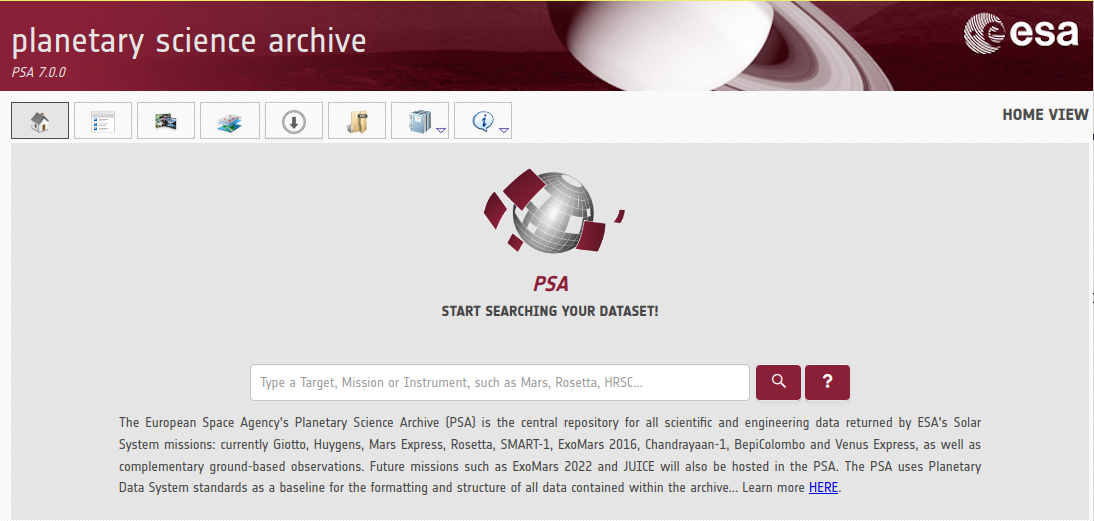
\includegraphics[width=\hsize]{form-psa}\\
        \vspace{1.0em}
          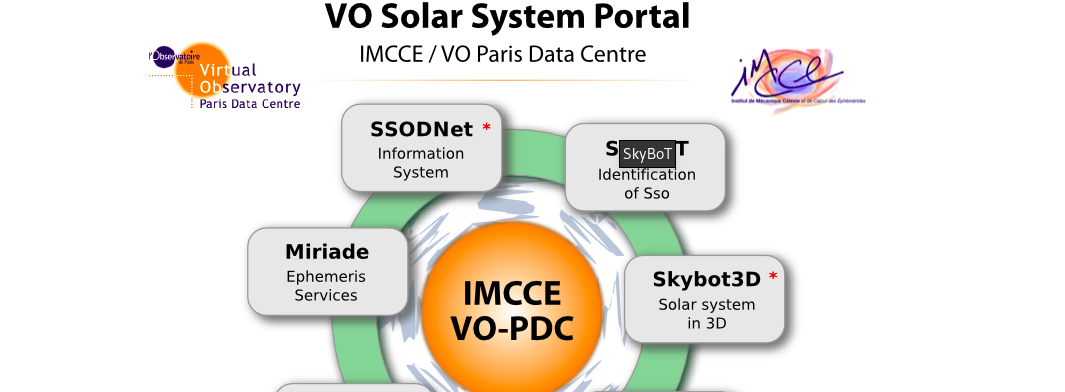
\includegraphics[width=\hsize]{portal-imcce}
        \end{onlyenv}

        \begin{onlyenv}<2>
        \end{onlyenv}

        \begin{onlyenv}<3>
        \end{onlyenv}

      \end{overlayarea}
    \end{column}

  \end{columns}

\end{frame}
%%%%%%%----  END  ----  ----%%%%%%


